\section{Muon System}
\label{sec:muonsystem}
The detection of muons is a powerful tool at hadron colliders because they leave a unique signal in the detector.
The signal is unique for a couple of reasons:
\begin{itemize}
\item A muon is charged so a muon's momentum can be measured via its trajectory.
\item A muon is a minimum ionizing particle so it will be one of the few particles that does not leave much energy in the calorimeter systems.
\end{itemize}
The muon system for the CMS detector is situated in the iron return yoke of the solenoid. 
Although the components of the muon system are different than that of the tracking system, it reconstructs charged particle tracks in a similar manner.
Being situated outside of the calorimeters and solenoid, all other particles that would otherwise interact with the muon system are stopped before reaching it.
A muon can be identified by matching a track in the inner tracking system to a track in the muon system.
Further, a muon can be more cleanly identified by restricting the amount of energy deposited near the muon in either of the calorimeters.

In the barrel region ($|\eta| < 1.2$) the muon system is primarily composed of Drift Tube (DT) chambers.
A drift tube is constructed by running a wire carrying a positive current through a tube filled with an inert gas.
When a charged particle enters the tube it will ionize the gas and the free electrons will be attracted to the wire, generating a signal that can be measured.
In the case of the CMS detector DTs, the gas is a mixture of 85\% Argon/15\% Carbon Dioxide, and the wires are held at a voltage of $3.6$ kV.
The muon barrel DT system is separated into five wheels each with four concentric layers where the inner three layers measure track positions in $r$, $\phi$ and $z$, while the outer most layer does not measure the $z$ coordinate.
The three inner cylinders are comprised of 60 drift chambers while the outer cylinder consists of 70 drift chambers for a total of approximately $172,000$ sensitive wires. 
A schematic of a muon DT wheel is shown in Figure \ref{fig:dtlayout}.
\begin{figure}[htpb]
\begin{center}
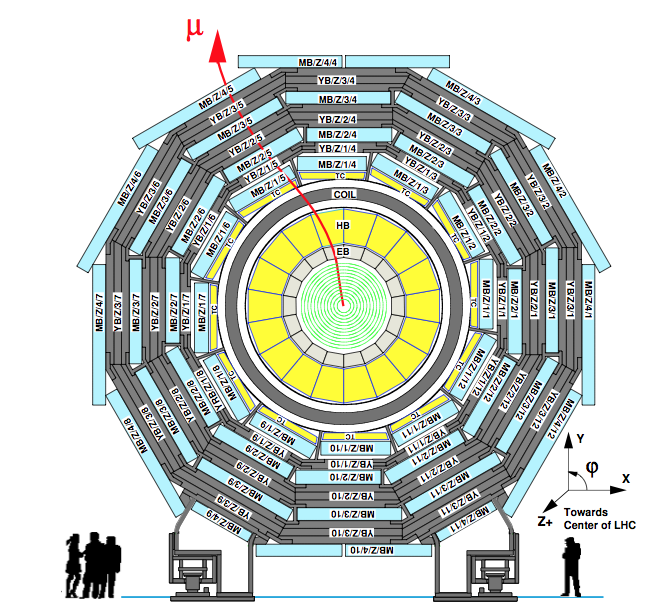
\includegraphics[width=0.9\textwidth]{plots/dtlayout.png}
\caption{Schematic of the CMS barrel muon DT chambers\cite{CMS_DETECTOR}.}
\label{fig:dtlayout}
\end{center}
\end{figure}

Cathode strip chambers (CSC) are used in the endcap regions, extending the coverage to $|\eta| < 2.4$. 
The CSC detectors are trapezoidal chambers filled with an inert gas.
Each chamber contains a plane of cathode strips organized radially, and a plane of anode wires held at high voltage running nearly perpendicular to the strips.
When a muon passes through one of the cathode strip chambers it will ionize the gas.
Once the gas has been ionized, an avalanche current will be created between an anode wire and a number of the cathode strips which can then be measured.
Using the measurement of the signal on the anode wire provides a signal that is fast enough to be used as a trigger sample, however, yields the relatively poor $r-\phi$ spatial resolution of $2$ mm.
The offline reconstructed position of the muon can be measured much more precisely by taking the average of the charge distribution on the cathode strips and the position of the anode wire.
Using the cathode strips as well as the anode wires provides a spatial resolution of $75$ \micrometer in the first layer and $150$ \micrometer in the outer layers.
The CSCs are distributed in the endcap region such that each chamber covers either $10^{\circ}$ or $20^{\circ}$ in $\phi$ and overlap to eliminate any gaps in $\phi$ coverage for the system.
The layout for the CSCs can be seen in Figure \ref{fig:csclayout}.
\begin{figure}[htpb]
\begin{center}
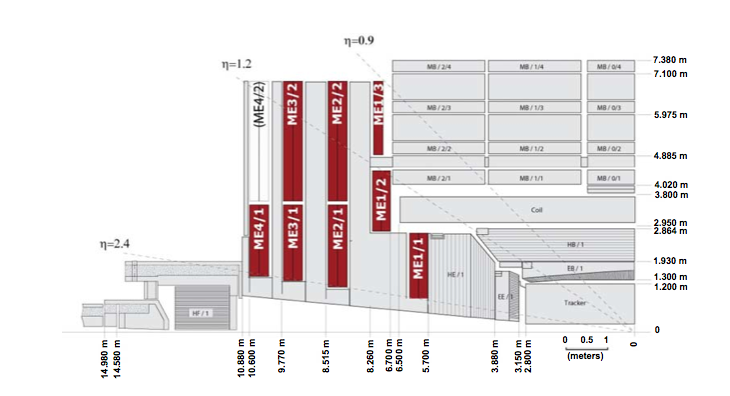
\includegraphics[width=0.9\textwidth]{plots/csclayout.png}
\caption{Schematic of the CMS muon system with the CSC chambers highlighted in red\cite{CMS_DETECTOR}.}
\label{fig:csclayout}
\end{center}
\end{figure}


As both the DT and CSC muon sub systems are relatively slow compared to the speed needed for the trigger system to correctly identify the associated bunch crossing with a triggered muon, an additional sub system exists to provide the muon system with the capability of providing a fast first level trigger.
The Resistive Plate Chamber (RPC) is a gaseous parallel-plate detector that provides a time resolution comparable to that of a scintillator\cite{RPC}.
The muon RPCs extend to $|\eta| \le 1.6$ covering the muon system barrel region and a portion of the endcap region. 
The layout of the RPCs is shown in Figure \ref{fig:rpclayout}.
The RPCs are capable of providing an estimate of the transverse momentum for a muon on a very short time scale that can unambiguously be matched to a bunch crossing even in the presence of the high rates and pile-up seen at the LHC.
Each chamber consists of two gaps (up/down) of $2$ mm operated in avalanche mode with a common read out strip between them, this provides a higher efficiency than would be obtainable with a single gap while allowing for a lower operating voltage. % FIXME MORE EXPLANATION
The RPC chambers utilize a gas mixture of $96.2\%$ \ce{C2H2F4}, $3.5\%$ \ce{iC4H10}, and $0.3\%$ \ce{SF6}.
% FIXME radiation?
\begin{figure}[htpb]
\begin{center}
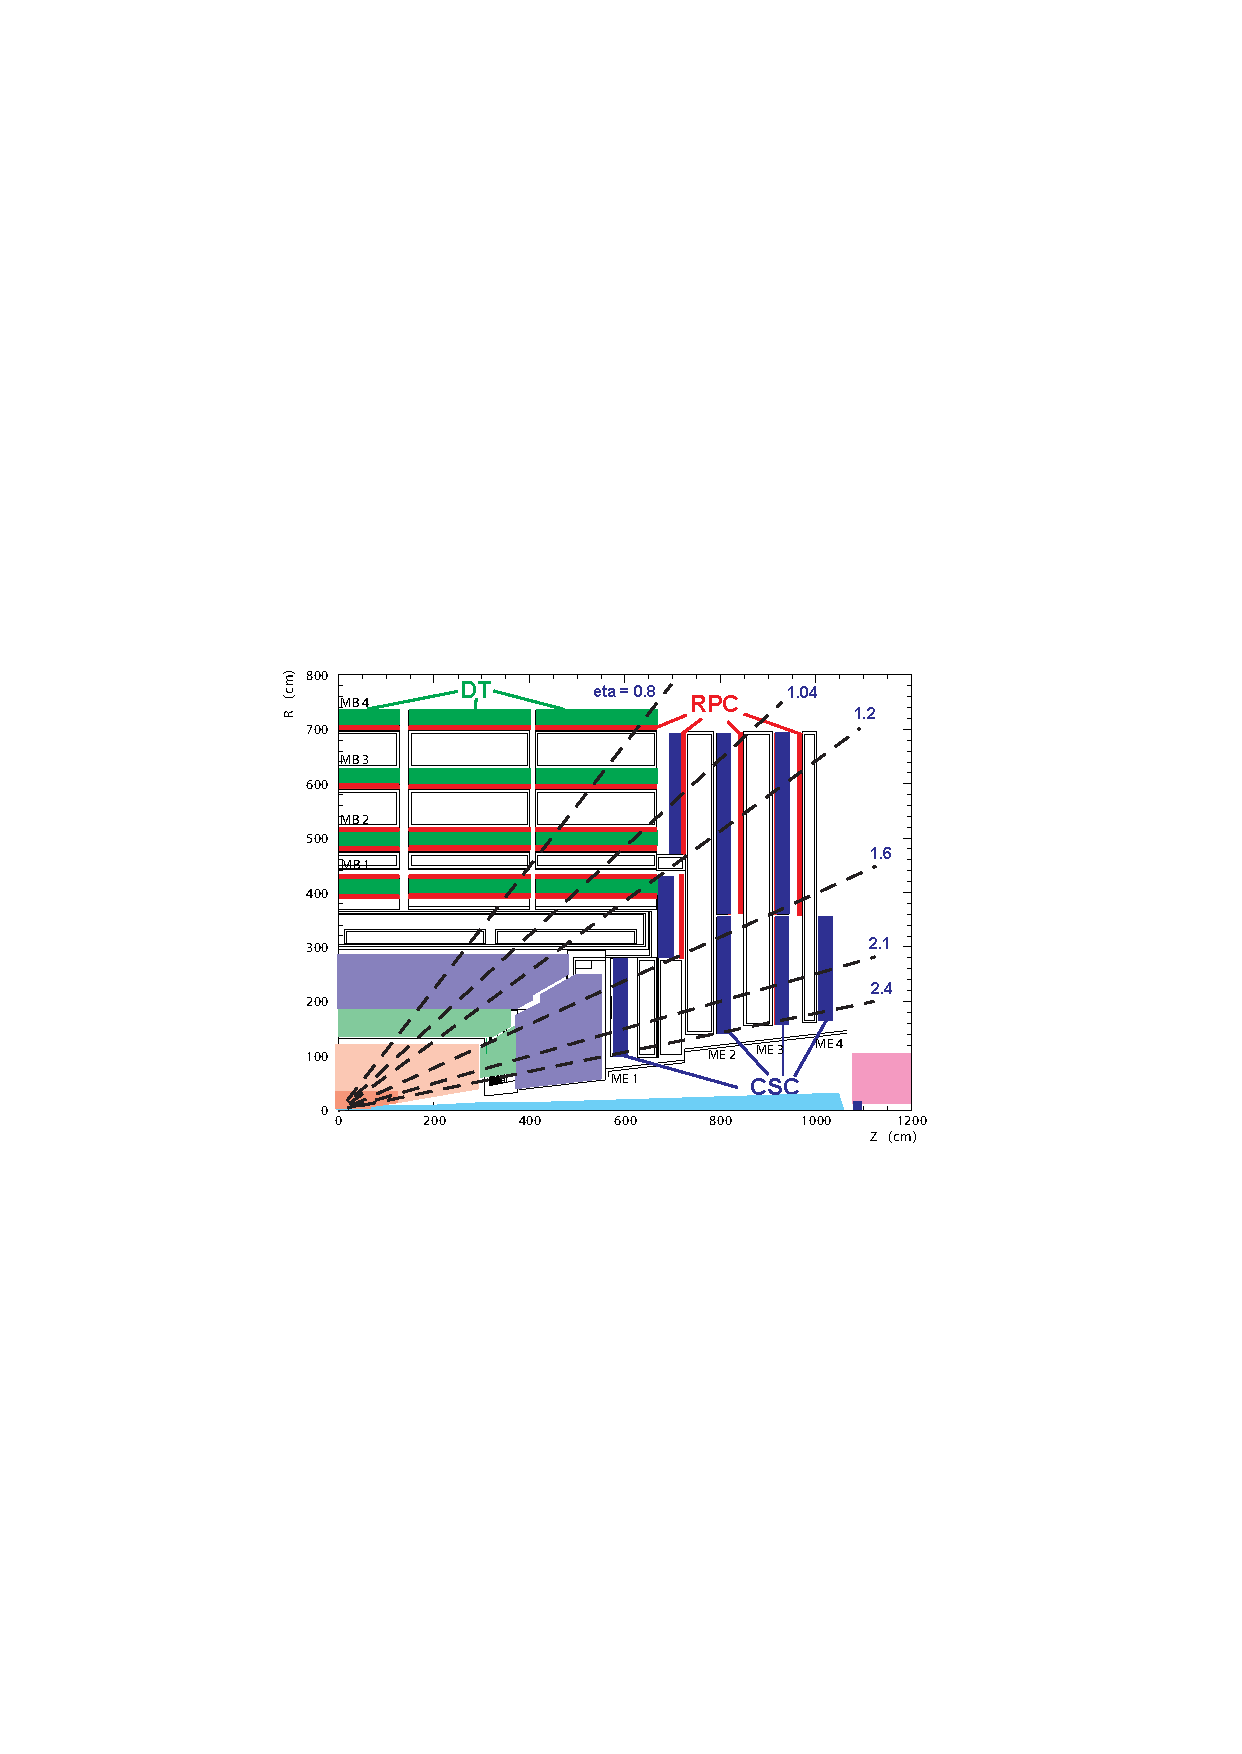
\includegraphics[width=0.9\textwidth]{plots/rpclayout.pdf}
\caption{Schematic of the CMS muon system\cite{TDR}.}
\label{fig:rpclayout}
\end{center}
\end{figure}

The resolution of muon momentum measurements suffers from multiple scattering in the detector material before the muon system.
The momentum resolution of the muon system is in the range of approximately $9\%$-$45\%$ depending on the $p$ and $\eta$.
This situation can be vastly improved, however, by performing a global momentum fit to the track measured in the inner tracker with the track measured in the muon system.
Figure \ref{fig:muonres} shows that the momentum resolution is improved by an order of magnitude for low $p_{T}$ and $\eta$ with a substantial improvement for high $p_{T}$ and $\eta$. 
In addition to performing a global fit, two independent measurements of the muon $p_{T}$ can provide a useful cross-check on the measured momentum.
\begin{figure}[htpb]
\begin{center}
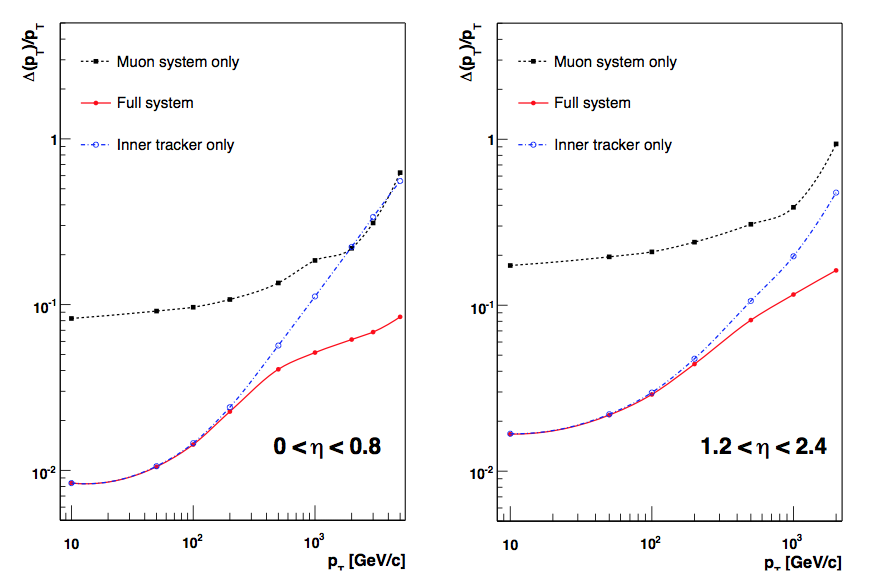
\includegraphics[width=0.9\textwidth]{plots/muonres.png}
\caption{Comparison of muon momentum resolution using the inner tracking system alone, the muon system alone, and the inner tracking system combined with the muon system for the barrel (left) and endcap (right) regions\cite{CMS_DETECTOR}.}
\label{fig:muonres}
\end{center}
\end{figure}

% RPC
